\begin{exercise}
The Bellman equation \eqref{eq:2.14} must hold for each state for the value function $v_\pi$ shown in Figure \ref{fig:2.14} (right). %of Example 3.5.
Show numerically that this equation holds for the center state, valued at $+0.7$, with respect to its four neighboring states, valued at $+2.3$, $+0.4$, $-0.4$, and $+0.7$.
(These numbers are accurate only to one decimal place.)

\begin{figure}[H]
    \centering
    \subfloat
    {
        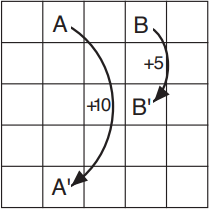
\includegraphics[width = 0.2 \textwidth]{2.14.1.png}
    }
    \hspace{1cm}
    \subfloat
    {
        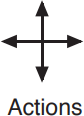
\includegraphics[width = 0.075 \textwidth]{2.14.2.png}
    }
    \hspace{1cm}
    \subfloat
    {
        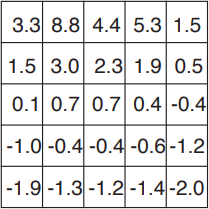
\includegraphics[width = 0.2 \textwidth]{2.14.3.png}
    }
    \hspace{0mm}
    \caption
    {
        Gridworld example:
        exceptional reward dynamics (left) and state-value function for the equiprobable random policy (right).
    }
    \label{fig:2.14}
\end{figure}

\begin{align} \label{eq:2.14}
    v_\pi(s)
    \doteq
    \sum_a
        \pi(a \mid s)
        \sum_{s^\prime, r}
            p(s^\prime, r \mid s, a)
            \bbraces{r + \gamma v_\pi(s^\prime)},
    \quad
    ~\text{for all}~ s \in \mathcal S
\end{align}

\end{exercise}

\begin{solution}
  We give the the states the names $m, u, d, l, r$ (for mid, up, down, left, right with respect to the state valued at $0.7$) and the actions $north, east, south, west$. According to the policy $\pi(a \mid m) = 0.25$ for all the actions $a$. Once we take an action the four argument function $p(s^\prime, 0 \mid m, a) = 1$ for exactly one pair of $(s^\prime, a)$ and $0$ otherwise. If we omit all the pairs with probability $0$ we get:

  \begin{align*}
    &\pi(north\mid m) p(u,0\mid m, north)[0 + \gamma v_\pi(u)]
    +
    \pi(east\mid m) p(l, 0 \mid m, east)[0 + \gamma v_\pi(l)] \\
    +
    &\pi(south\mid m) p(d,0\mid m, south)[0 + \gamma v_\pi(d)]
    +
    \pi(west\mid m) p(r, 0 \mid m, west)[0 + \gamma v_\pi(r)] \\
    =&
    0.25 \cdot\big([0.9\cdot 2.3] + [0.9\cdot 0.4] - [0.9\cdot 0.4] + [0.9\cdot 0.7]\big)
    =
    0.675
    \approx
    0.7
    =
    v_\pi(m)
  \end{align*}
\end{solution}
